\chapter{SKF}
\label{chap:skf}

\section{Introduzione}
SKF è un'azienda multinazionale specializzata nella produzione di cuscinetti a sfera. A seguito della formalizzazione del progetto Beat 4.0 portato avanti da SKF e ALTEN è iniziato un progetto di digitalizzazione degli impianti di produzione attraverso l'installazione di sensori all'interno dei macchinari lungo la catena di montaggio.
Il processo di produzione è composto da varie fasi e parte da due anelli grezzi che costituiranno le parti interne ed esterne del prodotto finale. Entrambi gli anelli vengono raffinati in parallelo attraverso due operazioni sequenziali: la rettifica e la levigatura. 
I due anelli vengono poi assemblati insieme ad altri componenti come la gabbia e gli elementi di rotolamento. Il prodotto finito passa infine attraverso un macchinario il quale esegue misure per valutarne la qualità. 

I dati prodotti dai macchinari sono quindi divisi in due categorie: 
\begin{itemize}
	\item \textbf{CoMo}: dati relativi ai sensori installati sui macchinari di rettifica e levigatura cui fanno riferimento a vibrazione, temperatura, velocità, pressione e scorrimento.
	\item \textbf{MVM}: sono i dati prodotti dai macchinari di controllo qualità sul prodotto finito.
\end{itemize}

Lo scopo di questo progetto e di questa tesi è quello di applicare tecniche non supervisionate di rilevamento anomalie utilizzando i dati a disposizione prodotti dai sensori installati sui macchinari.

\section{Descrizione del dataset}
Poiché i dati sono di proprietà della SKF, la descrizione è ridotta e i nomi delle misure e delle macchine sono fittizi.


\subsection{CoMo}
I dati includono le misurazioni di differenti caratteristiche di alcune delle macchine della catena di produzione. Per ogni macchina monitorata, sono incluse le velocità radiali e assiali, gli inviluppi radiali e assiali, la temperatura, pressione e vibrazione.
Poiché non tutte le macchine dell'impianto sono monitorate vengono persi dettagli e completezza nei dati, ma nonostante questo il dataset a disposizione contiene una grande quantità di dati.
La frequenza di registrazione dei dati CoMo è di 10 minuti. Questo valore così basso porta con se delle problematiche che verranno discusse più avanti, per questo motivo si sta cercando per richiedere di alzare la frequenza.

\subsection{MVM}
I dati di qualità vengono registrati per ogni prodotto che esce dalla catena di produzione.
Le misure di qualità fornite sono quattro fasce, indicate con A, B, C e D.
Tutte le fasce sono positive per definizione ed ognuna di esse tratta uno specifico tipo di difetto in ogni cuscinetto attraverso l'analisi dello spettro. In particolare:
\begin{itemize}
	\item Banda A riguarda i cosiddetti errori geometrici risultanti dalla fase di rettifica.
	\item Banda B e C riguardano errori nella fase di levigatura.
	\item Banda D trova errori causati dalla presenza di impurità negli oli o liquidi di pulizia usati sui cuscinetti.
\end{itemize}

Considerato la frequenza di uscita di prodotti finiti dalla linea di produzione, i dati MVM sono prodotti ogni due secondi. Questi verranno poi aggregati in intervalli di 10 minuti. La scelta di dieci minuti per la lunghezza del gap temporale non è casuale, infatti è stata fatta per adattarsi alla granularità dei dati CoMo.

\subsubsection{Qualità}
I dati di qualità MVM vengono usati per definire la classe di qualità di appartenenza dei cuscinetti a sfera. Per fare ciò, sono state definite per ogni banda delle soglie alla quale il superamento di una porta il prodotto a ricevere una classificazione di qualità più bassa.
La tabella \ref{mvm-soglie} mostra come le classi di qualità vengano definite. Per questioni di riservatezza vengono mostrati dei valori di soglia modificati, andando a moltiplicare i valori reali per uno scalare.

\begin{table}
	\caption{\label{mvm-soglie}Soglie bande MVM.}
	\centering
	\begin{tabular}{|l|l|l|l|l|}
		\hline
		Classe & \multicolumn{1}{c|}{Banda A} & \multicolumn{1}{c|}{Banda B} & \multicolumn{1}{c|}{Banda C} & \multicolumn{1}{c|}{Banda D} \\ \hline
		Q1     & 25                           & 7.2                          & 7.2                          & 3.6                          \\ \hline
		Q2     & 36                           & 18.2                         & 18.2                         & 5.2                          \\ \hline
		Q3     & 48                           & 25.6                         & 25.6                         & 12                           \\ \hline
		Q4     & 72                           & 36                           & 36                           & 20                           \\ \hline
	\end{tabular}
\end{table}

Valori di banda più bassi indicano una qualità maggiore, di conseguenza la classe Q1 rappresenta i prodotti migliori mentre la classe Q4 rappresenta gli scarti. 
Per passare da una classe alla successiva è necessario che solamente una delle 4 bande superi il valore di soglia. 
La tabella \ref{mvm-esempio} mostra un esempio di come le classi vengano computate.

\begin{table}
	\caption{\label{mvm-esempio}Esempio di associazione di Classe qualità.}
	\centering
	\begin{tabular}{|l|l|l|l|l|l|}
		\hline
		Bearing & \multicolumn{1}{c|}{Banda A} & \multicolumn{1}{c|}{Banda B} & \multicolumn{1}{c|}{Banda C} & \multicolumn{1}{c|}{Banda D} & Qualità \\ \hline
		B1      & 20                           & 7                            & 4                            & 2                            & Q1      \\ \hline
		B2      & 19                           & 18                           & 2                            & 5.8                          & Q3      \\ \hline
		B3      & 70                           & 20                           & 20                           & 18                           & Q4      \\ \hline
	\end{tabular}
\end{table}

\section{Processamento dei dati}
I dati sono ricevuti da SKF in formato tabellare e sono suddivisi in dati CoMo e dati MVM. Ogni riga della tabella della qualità corrisponde a un cuscinetto analizzato dalla macchina di qualità, invece le colonne sono costituite dalla data e ora di registrazione dei valori e dalle quattro bande.
La tabella CoMo invece contiene le misure del Condition Monitoring in formato non pivotante: ogni riga corrisponde a un singolo record contenente l'ora del record, il nome della macchina a cui il record si riferisce, il nome della feature misurata e il valore registrato.

Considerando il formato grezzo dei dati, è necessario eseguire diverse trasformazioni per produrre dati pronti al processamento da parte di algoritmi di Machine Learning. 

Prima di entrare nel dettaglio è però necessario condividere alcune osservazioni sulle proprietà dei dati.

\subsection{Proprietà}

\subsubsection{Parzialità dei dati}
Come già detto, solo una parte delle macchine del canale viene monitorata.
In particolare, per il processamento dell'anello esterno i dati vengono raccolti solamente dalle macchine di rettifica, mentre l'operazione di levigatura è completamente inaccessibile.
Per quanto riguarda l'anello interno, l'operazione di levigatura viene eseguita da due macchine che lavorano in parallelo su anelli diversi. Una di queste due è dotata di sensori, mentre l'altra no. Le macchine di rettifica sono invece tutte monitorate.
Non vengono registrati dati per l'assemblaggio dei cuscinetti e solamente una delle due macchine di qualità poste in parallelo produce e condivide i dati che registra. Solitamente la divisione del lavoro delle due macchine di qualità non è esattamente 50/50, ma a lavorare è soltanto quella mappata. Per cui i dati sulla qualità sono disponibili per tutti i cuscinetti a sfera tranne in casi specifici in cui la macchina registrata viene interrotta per manutenzione.

\subsubsection{Frequenza di registrazione}
I vari tipi di sensori non registrano con la stessa frequenza di registrazione e allo stesso momento.
È quindi necessario appiattire i timestamp e aggregare alcuni dati per fare in modo che ogni riga corrisponda alle misure di tutti i sensori monitorati nel periodo di riferimento.


\subsubsection{Frequenza di produzione}
La frequenza di produzione cambia nel tempo. Se vengono aggregati i dati di qualità con intervalli di tempo di 10 minuti, il numero di registrazioni in ogni intervallo è la quantità di cuscinetti analizzati dal monitoraggio.
Poiché ogni cuscinetto prodotto passa attraverso le macchine di qualità, questa quantità è ovviamente correlata alla velocità media di produzione
lungo l'intervallo di tempo considerato. 

Il motivo principale per cui la velocità media di produzione è interessante è che può essere utilizzata come indicatore del fatto che il canale è stato inattivo lungo nell'intervallo di dieci minuti considerato. In particolare, se la velocità media di produzione di un intervallo è significativamente più piccola del solito, indicherà che la produzione è stata interrotta nel periodo considerato. Le possibili cause di tale sospensione possono essere un malfunzionamento, la manutenzione o anche la chiusura programmata del canale.
Per quanto riguarda la quantità di cuscinetti analizzati dalla macchina di qualità monitorata, è vero che, se il processo di produzione è stato sospeso, questa quantità sarà bassa, ma non si può dire con certezza l'opposto.
Questa misura fornisce comunque alcuni indizi sull'attività del canale. Per esempio, esplorando il set di dati, si può notare che la quantità menzionata vada a zero ogni domenica dalle 12:00 alle 22:00 circa, conseguenza del fatto che in quel periodo di tempo c'è stato un turno di riposo. Questo viene confermato anche analizzando i dati CoMo nello stesso periodo temporale: numerosi sensori che producono valori a 0 oppure non li producono affatto, mentre quelli della temperatura iniziano a declinare. 

Queste osservazioni possono essere utilizzate per rilevare i turni di riposo e potenzialmente anche per le fasi di manutenzione, anche se per questi ultimi la rilevazione è di fatto impossibile. In particolare, le manutenzioni sono state registrate su carta, per cui non è possibile sfruttare questi dati come risposta e di conseguenza non è possibile convalidare statisticamente alcuna ipotesi.
Inoltre, la maggior parte delle manutenzioni dura meno di 10 minuti e
non disponendo di dati ad alta frequenza, è quasi sempre impossibile
osservare qualsiasi cambiamento nel comportamento delle serie temporali CoMo. 

\subsubsection{Dati Mancanti}
Per alcuni sensori sono disponibili solo poche settimane di dati e di conseguenza devono essere scartati. Per la parte restante dei dati, escludendo i tempi di inattività, in media il 15\% dei sensori è mancante in un dato momento e ogni misura è mancante in media il 17\% delle volte. Considerato anche quanto detto nel paragrafo precedente, esistono diverse cause possibili per cui un sensore non registra alcun valore in un dato momento. Per esempio, un errore nella configurazione dei sensori, è in corso il turno di riposo ed è possibile che lo stesso accada anche durante le manutenzioni o i crash della macchina.
In generale, non è chiaro come questi eventi possano influenzare l'attività dei sensori. D'altra parte, i sensori potrebbero essere semplicemente mal funzionanti o instabili, così come ci potrebbero essere problematiche nella memorizzazione dei dati all'interno del server locale. 
In conclusione, riuscire a decodificare le reali motivazioni per cui si ha una mancata registrazione potrebbe migliorare in maniera significativa le performance di algoritmi di Machine Learning. Purtroppo a causa della bassa frequenza di registrazione e data la non possibilità di interagire o comunicare con i tecnici dell'impianto di produzione, sono state messe in atto solamente delle semplici operazioni di processamento.

\subsubsection{Andamento Serie Temporali}
Le serie temporali di SKF presentano un comportamento stabile nel tempo. Come mostrato in figura \ref{sensors_plot}, elementi di stagionalità non sono presenti e non vi è presenza di trend e quindi le serie possono riferirsi stazionarie. Ipotesi confermata anche dall'esecuzione del test Augmented Dickey-Fuller nel quale veniva rifiutata la Null Hypothesis (la Null Hypothesis affermava la NON stazionarietà dei dati).
Per questo motivo, nelle fasi di processamento, operazioni di decomposizione delle serie temporali non sono state fatte.
È possibile comunque notare un'alta variabilità dei dati all'interno della singola serie temporale, con fluttuazioni più o meno visibili.
\begin{figure}[t]
	\centering
	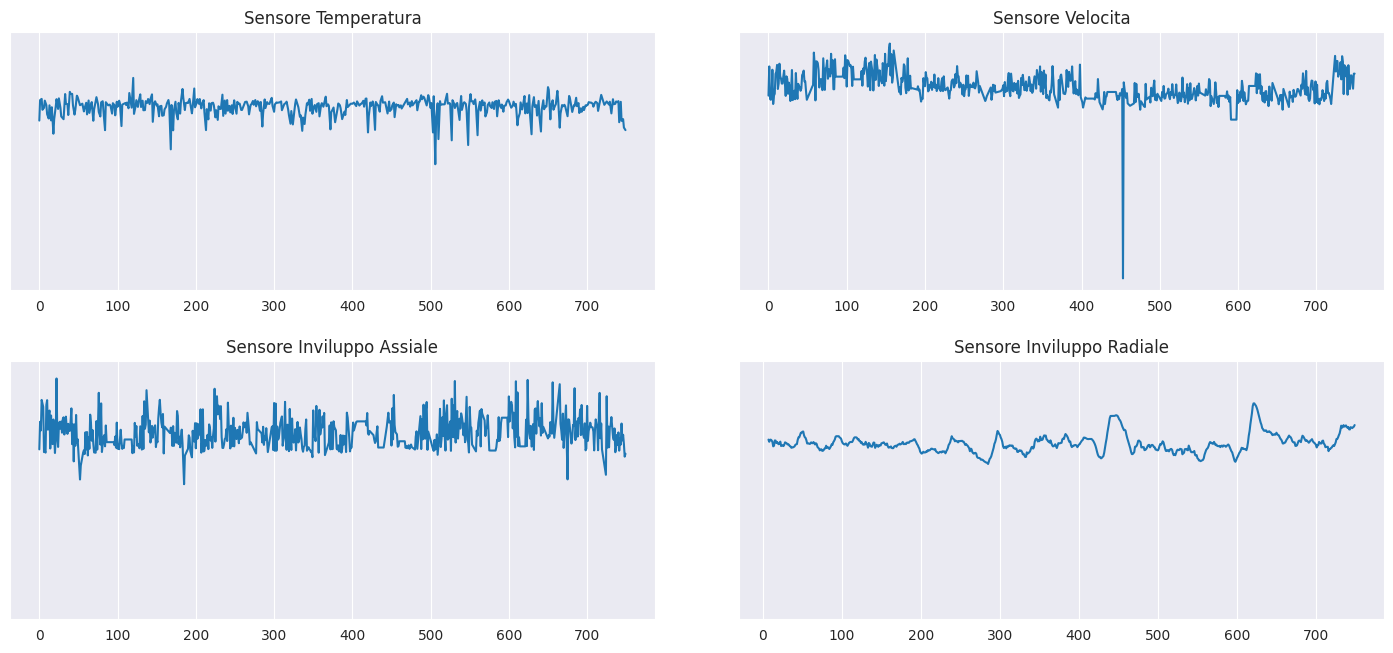
\includegraphics[width=14cm, scale=1]{images/sensors_plot}
	\caption{Andamento Serie Temporali}
	\label{sensors_plot}
		
\end{figure}

\subsection{Processamento}
Evitando i dettagli per questione di riservatezza, in questa sezione vengono presentati i passaggi principali eseguiti per produrre i set di serie temporali dai dati grezzi ricevuti da SKF. 
Per creare una tabella contente una colonna per ogni sensore e con un indice temporale è necessario appiattire i timestamp fino a raggiungere una granularità di 10 minuti, in modo che il tempo possa essere utilizzato come chiave per l'unione. A questo punto ogni riga del dataset corrisponde a un'istantanea di un particolare sensore anche se questa è chiaramente un'approssimazione: in pratica, le registrazioni di misure CoMo diverse non avvengono nello stesso istante, ma la maggior parte di esse si concentra in un intervallo di un minuto circa. 
D'altra parte, i dati sulla qualità sono raccolti in tempo reale quando viene analizzato ogni cuscinetto. In questo caso è quindi necessario aggregare questi dati secondo una qualche misura ed è stata scelta l'operazione di media.
Chiaramente, i dati MVM forniscono informazioni sull'intero intervallo di tempo mentre dati CoMo forniscono invece un'istantanea all'interno dell'intervallo di tempo.
Nell'unire queste misure si è ipotizzato che l'istantanea sia rappresentativa dell'intervallo di tempo ma a causa dell'alta variabilità della maggior parte delle serie temporali, questa ipotesi è lontana dalla realtà.
Questa condizione è molto distante da una situazione ottimale, per questo motivo si sta cercando per spingere a portare la frequenza di registrazione ad uno al minuto. Frequenze più alte consentiranno all'ipotesi sopra descritta di essere valida.

Allo stesso modo in cui sono stati aggregati i dati MVM, può capitare anche all'interno dei dati CoMo che più record dello stesso sensore possano ricadere nello stesso intervallo di tempo. In questo, per ogni tipologia di sensore è stata scelta una funzione di aggregazione tra massimo, minimo e media. La scelta è stata fatta pensando a quali potessero essere i valori più informativi per la caratteristica. Ad esempio, le pressioni sono state sono state aggregate con la funzione di massimo, poiché è probabile che le anomalie siano dei valori elevati; mentre per i flussi è stata scelta la funzione di minimo. Nei casi dubbi l'aggregazione è stata effettuata attraverso la funzione di media.

Dopo i passaggi precedenti, è possibile fare il pivoting della tabella CoMo  prendendo il timestamp come indice di riga. Il risultato è una tabella in cui ogni colonna corrisponde a una serie temporale. 
Come passo finale è necessario trattare i valori mancanti:
\begin{itemize}
	\item Nel caso di intervalli più lunghi di 8 ore con almeno il 50\% di valori mancanti, questi vengono eliminati dal dataset. L'obiettivo è quello di pulire il dataset dai dati registrati durante i turni di riposo in quanto non è di nostro interesse rilevare anomalie in quei intervalli di tempo.
	\item Tutti gli altri valori nulli vengono interpolati linearmente.
\end{itemize}
A questo punto i sensori vengono raggruppati per macchinario, andando quindi a produrre una tabella per ogni macchina.
Come ultimo passaggio si è deciso di andare a normalizzare i valori utilizzando un MinMax Scaler. Questa tecnica permette di normalizzare i valori passando il range del codominio della funzione come parametro di input, in questo caso [0,1]. La formula è definita come:
\[X_{scaled} = (X - X.min(axis=0)) / (X.max(axis=0) - X.min(axis=0))\]

Il valore originario massimo assumerà valore 1, quello minimo 0 e tutti gli altri un valore compreso.